\section{Results}
\label{sec:results}

\subsection{Part 1}

\paragraph{Cluster diagnostics} (\cref{fig:kmeans}).
Inertia falls smoothly with no elbow.
Silhouette is lowest at $K=3$ (0.163) and rises to 0.307 at $K=80$ without a peak.
Purity rises from 0.583 to 0.872, but 0.583 at $K=2$ is exactly the purity of predicting Recruitment for every trial.
ARI peaks at $K=5$ (0.203) and falls to 0.076 at $K=80$.
Larger $K$ therefore produces smaller pieces, not partitions closer to the reasons.
In the PCA projection (\cref{fig:pca}), the four minority reasons overlap in one region while Recruitment spreads over the whole plot.

\begin{figure*}[t]
\centering
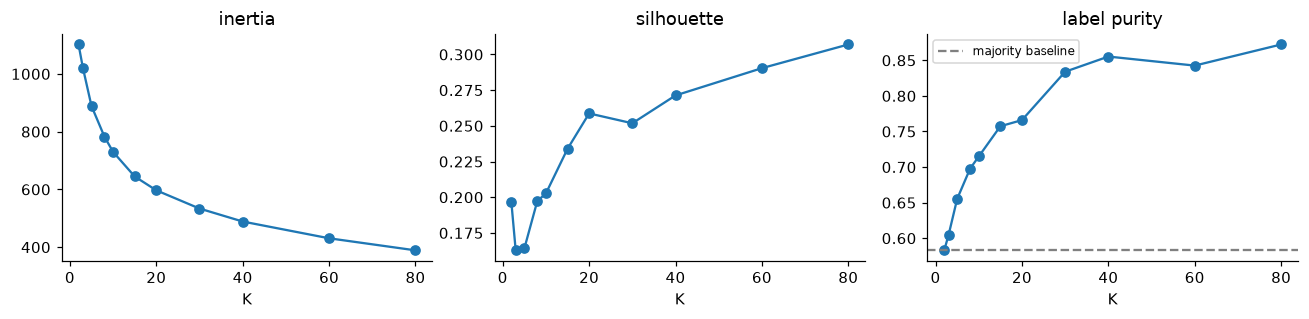
\includegraphics[width=0.9\textwidth]{fig/p1_kmeans_diag.png}
\caption{K-means on all 1,561 trials: inertia, silhouette and label-set purity. Dashed line: purity of predicting Recruitment for every trial (0.583).}
\label{fig:kmeans}
\end{figure*}

\begin{figure}[t]
\centering
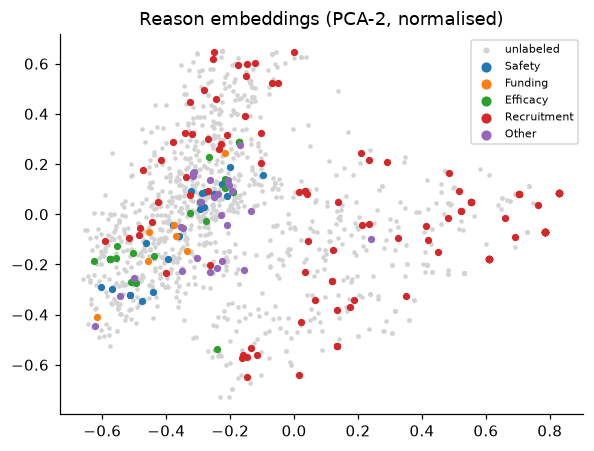
\includegraphics[width=0.78\linewidth]{fig/p1_pca2.png}
\caption{PCA of the L2-normalized reason embeddings. Colored points are single-reason labeled trials; all others are grey.}
\label{fig:pca}
\end{figure}

\paragraph{Method comparison.}
\Cref{tab:p1} lists one configuration per family; all 40 are in the notebook.
The supervised LR is insensitive to $C$ (validation sample-F1 0.859--0.872).
B improves with $K$ (0.801 at $K=10$ to 0.844 at $K=80$), and B0 gets Funding F1 $=0$ at $K=10$ and 20.
E0 gets worse as $\lambda$ grows: for $d=10$, validation sample-F1 falls from 0.868 to 0.724 and CV from 0.845 to 0.806 as $\lambda$ goes from 0 to 1.
Raising E's threshold from 0.8 to 0.95 changes validation sample-F1 only from 0.838 to 0.844.
F at threshold 0.8 reaches 0.895 / 0.769, close to the best C configuration (0.893 / 0.785 at $K=10$).
With $d=20$ and $\lambda=1$, EM converges after 70 iterations, and 91.1\% of unlabeled trials then have a maximum posterior of at least 0.95 (\cref{fig:ssgmm}).

\begin{table}[t]
\centering
\footnotesize
\setlength{\tabcolsep}{3.5pt}
\begin{tabular}{@{}lcccc@{}}
\toprule
Method & val s-F1 & val m-F1 & CV s-F1 & CV m-F1 \\
\midrule
Baseline (starter code) & 0.8654 & 0.7067 & -- & -- \\
A supervised LR ($C=0.1$) & 0.8590 & 0.7291 & \textbf{0.8957} & \textbf{0.7979} \\
B0 K-means vote ($K=40$) & 0.8462 & 0.6844 & 0.8195 & 0.6469 \\
B K-means pseudo ($K=40$, $w_u=0.3$) & 0.8162 & 0.6963 & 0.8579 & 0.7347 \\
C K-means $\cap$ LR ($K=20$) & 0.8761 & 0.7709 & 0.8818 & 0.7688 \\
D GMM soft labels ($K=20$) & 0.7744 & 0.6174 & 0.7924 & 0.6305 \\
E ss-GMM pseudo ($d=20$, 0.95) & 0.8440 & 0.6936 & 0.8630 & 0.7074 \\
F self-training (0.95) & 0.8654 & 0.7578 & 0.8818 & 0.7817 \\
G label spreading ($k=20$) & 0.6923 & 0.4816 & 0.8319 & 0.5843 \\
\textbf{H ensemble (A+C+E)} & \textbf{0.8974} & \textbf{0.8058} & 0.8900 & 0.7714 \\
\bottomrule
\end{tabular}
\caption{Part 1 validation and 2$\times$5-fold CV results. s-F1: sample-wise F1; m-F1: macro-F1.}
\label{tab:p1}
\end{table}

\begin{figure}[t]
\centering
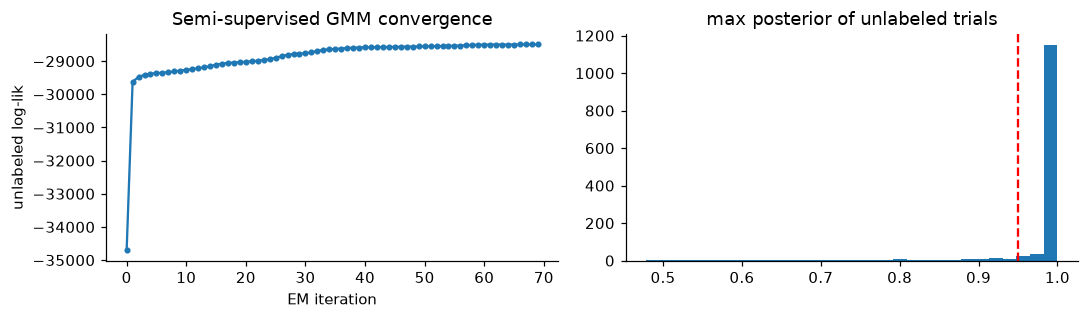
\includegraphics[width=\linewidth]{fig/p1_ssgmm.png}
\caption{Semi-supervised GMM: unlabeled log-likelihood per EM iteration (left) and maximum posterior of unlabeled trials after convergence (right, red line at 0.95).}
\label{fig:ssgmm}
\end{figure}

\paragraph{Selected model and features.}
H raises macro-F1 by 0.099, and Funding alone gains 0.464 (\cref{tab:perlabel}).
Among feature groups (\cref{tab:feat}), only text SVD helps, by 0.013 or about one validation trial, and adding all groups scores below text alone, so the final model uses the embeddings only.
Without year information, H predicts Safety for 0.183 of test trials against 0.102 in the labeled set, and Recruitment for 0.580 against 0.643.

\begin{table}[t]
\centering
\footnotesize
\setlength{\tabcolsep}{3pt}
\begin{tabular}{@{}lccccccc@{}}
\toprule
 & Safety & Funding & Efficacy & Recruit. & Other & s-F1 & m-F1 \\
\midrule
Baseline & 0.857 & 0.286 & 0.828 & 0.980 & 0.583 & 0.865 & 0.707 \\
H & 0.889 & 0.750 & 0.800 & 0.990 & 0.600 & 0.897 & 0.806 \\
\bottomrule
\end{tabular}
\caption{Per-label validation F1.}
\label{tab:perlabel}
\end{table}

\begin{table}[t]
\centering
\footnotesize
\begin{tabular}{@{}lccc@{}}
\toprule
Feature set & Dim. & val s-F1 & val m-F1 \\
\midrule
Embedding only (used) & 150 & 0.8590 & 0.7291 \\
+ \texttt{start\_year} & 151 & 0.8526 & 0.7462 \\
+ text TF-IDF $\rightarrow$ SVD-50 & 200 & 0.8718 & 0.7533 \\
+ drug match and actions & 180 & 0.8632 & 0.7335 \\
+ level-0 pathways & 179 & 0.8632 & 0.7453 \\
+ all & 260 & 0.8611 & 0.7492 \\
\bottomrule
\end{tabular}
\caption{Feature groups added to the supervised LR ($C=0.1$).}
\label{tab:feat}
\end{table}

\subsection{Part 2}

The selected model is the pooled field-wise TF-IDF LR with $C=1$.
It improves every metric in every phase (\cref{tab:p2main}), and mean log loss falls from 0.940 to 0.567.
\Cref{tab:p2all} lists representative configurations.

\begin{table}[t]
\centering
\footnotesize
\setlength{\tabcolsep}{2.5pt}
\begin{tabular}{@{}lcccc@{}}
\toprule
Phase & F1 & ROC-AUC & PR-AUC & Log loss \\
\midrule
I & .701 $\rightarrow$ .727 & .703 $\rightarrow$ .759 & .754 $\rightarrow$ .799 & .879 $\rightarrow$ .585 \\
II & .614 $\rightarrow$ .645 & .663 $\rightarrow$ .737 & .638 $\rightarrow$ .718 & 1.060 $\rightarrow$ .599 \\
III & .774 $\rightarrow$ .815 & .705 $\rightarrow$ .789 & .815 $\rightarrow$ .878 & .881 $\rightarrow$ .516 \\
Mean & .696 $\rightarrow$ .729 & .690 $\rightarrow$ .761 & .736 $\rightarrow$ .798 & .940 $\rightarrow$ .567 \\
\bottomrule
\end{tabular}
\caption{Validation results per phase, baseline $\rightarrow$ selected model.}
\label{tab:p2main}
\end{table}

\begin{table}[t]
\centering
\footnotesize
\setlength{\tabcolsep}{3pt}
\begin{tabular}{@{}lcccc@{}}
\toprule
Model (mean over phases) & F1 & AUC & PR-AUC & LL \\
\midrule
Ens.\ pooled + per-phase TF-IDF LR & .725 & .765 & .802 & .564 \\
Ens.\ pooled + kNN & .727 & .765 & .806 & .565 \\
\textbf{Pooled field-wise LR (selected)} & .729 & .761 & .798 & .567 \\
TF-IDF 1--2gram LR & .723 & .757 & .795 & .570 \\
Field-wise LR + Morgan & .718 & .753 & .798 & .575 \\
Field-wise LR & .722 & .755 & .799 & .576 \\
Field-wise LR + pathway/target/action & .715 & .753 & .798 & .576 \\
Field-wise LR + \texttt{start\_year} & .730 & .749 & .793 & .578 \\
BoW LR, $C=0.01$ & .733 & .737 & .779 & .592 \\
kNN, TF-IDF, $k=75$ & .718 & .734 & .779 & .598 \\
MNB, TF-IDF, $\alpha=1$ & .718 & .724 & .778 & .652 \\
Baseline: BoW LR, $C=1$ & .696 & .690 & .736 & .940 \\
MNB, counts, $\alpha=1$ & .701 & .714 & .737 & 3.651 \\
\bottomrule
\end{tabular}
\caption{Part 2 validation results, sorted by log loss (LL).}
\label{tab:p2all}
\end{table}

\paragraph{Error analysis} (\cref{tab:err,fig:err}).
The no-recorded-reason group holds 44\%, 54\% and 67\% of failed trials in phases I, II and III.

\begin{table*}[t]
\centering
\footnotesize
\setlength{\tabcolsep}{4pt}
\begin{tabular}{@{}l cccc cccc cccc@{}}
\toprule
 & \multicolumn{4}{c}{Phase I} & \multicolumn{4}{c}{Phase II} & \multicolumn{4}{c}{Phase III} \\
\cmidrule(lr){2-5}\cmidrule(lr){6-9}\cmidrule(l){10-13}
Group & $n$ & t/p & base & impr. & $n$ & t/p & base & impr. & $n$ & t/p & base & impr. \\
\midrule
Safety & 9 & 1/8 & .444 & .556 & 13 & 1/12 & .615 & .385 & 7 & 1/6 & .714 & .571 \\
Funding & 4 & 1/3 & .500 & .000 & 4 & 1/3 & .250 & .000 & 0 & -- & -- & -- \\
Efficacy & 2 & 0/2 & .500 & 1.00 & 11 & 0/11 & .273 & .455 & 9 & 0/9 & .667 & .778 \\
Recruitment & 23 & 2/21 & .391 & .391 & 88 & 12/76 & .352 & .239 & 21 & 5/16 & .571 & .667 \\
Other & 3 & 0/3 & .333 & .333 & 22 & 3/19 & .409 & .364 & 10 & 2/8 & .700 & .700 \\
No recorded reason & 28 & -- & .571 & .429 & 144 & -- & .375 & .306 & 82 & -- & .451 & .537 \\
\midrule
All failed & 64 & & .469 & .422 & 265 & & .370 & .283 & 123 & & .496 & .569 \\
\bottomrule
\end{tabular}
\caption{FPR of failed validation trials by reason group, baseline (base) and improved model (impr.). t/p: trials whose reason is a true label / a Part 1 prediction.}
\label{tab:err}
\end{table*}

\begin{figure*}[t]
\centering
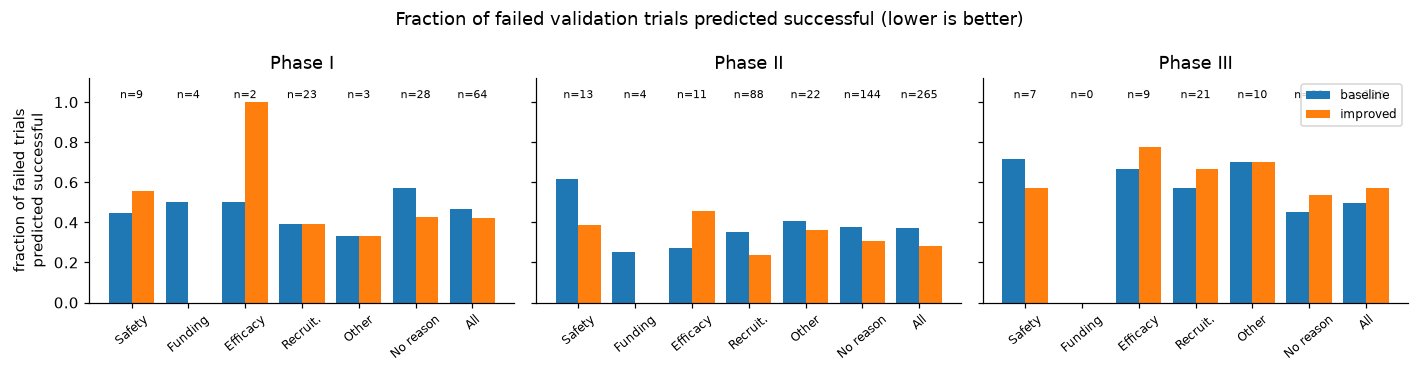
\includegraphics[width=0.9\textwidth]{fig/p2_err_compare.png}
\caption{FPR by reason group, baseline vs.\ improved model. Phase III has no Funding trials. The phase III legend hides two sizes: no recorded reason $n=82$, all failed $n=123$.}
\label{fig:err}
\end{figure*}

\paragraph{Trade-offs and drift.}
Raising the threshold from 0.5 to 0.7 cuts the phase II FPR from 0.283 to 0.083 but its F1 from 0.645 to 0.504 (\cref{tab:thr}).
\texttt{class\_weight="balanced"} moves mean AUC from 0.7612 to 0.7609 and log loss from 0.5665 to 0.5685, with slightly lower F1 in every phase.
Shrinkage is best at $s=1$ on both splits (temporal log loss 0.5672, 0.5683, 0.5717, 0.5772 for $s=1$ to 0.7).
Test predictions lie in $[0.080,0.979]$, so clipping changes almost nothing.
On the temporal split, the pooled LR's AUC falls from 0.761 to 0.695 with log loss 0.567 in both cases, while the baseline goes from 0.690 to 0.617 AUC and from 0.940 to 1.018 log loss.
Later trials succeed more often (0.655 against 0.522).

\begin{table}[t]
\centering
\footnotesize
\setlength{\tabcolsep}{3pt}
\begin{tabular}{@{}lccc@{}}
\toprule
Thr. & F1 I / II / III & FPR I / II / III & TPR I / II / III \\
\midrule
0.4 & .776 / .664 / .825 & .547 / .460 / .667 & .894 / .754 / .942 \\
\textbf{0.5} & .727 / .645 / .815 & .422 / .283 / .569 & .753 / .627 / .888 \\
0.6 & .693 / .608 / .800 & .234 / .128 / .415 & .624 / .500 / .808 \\
0.7 & .585 / .504 / .756 & .109 / .083 / .244 & .447 / .369 / .683 \\
\bottomrule
\end{tabular}
\caption{Selected model at different thresholds (0.5 used).}
\label{tab:thr}
\end{table}
